% GENERATED BY sshrc_figures.py - edit that file, not this one.
% The document that inputs this file supplies the float, the caption and the label.
% Stream B. Committees, left to right within each year: Philosophy, History, Fine arts, Literature, Sociology, Geography, Psychology (10A, 10B), Political science, Education (12A, 12B, 12C), Anthropology, Linguistics, Communications, Law and criminology.
\definecolor{sshrcA}{HTML}{2A78D6}
\definecolor{sshrcB}{HTML}{EB6834}
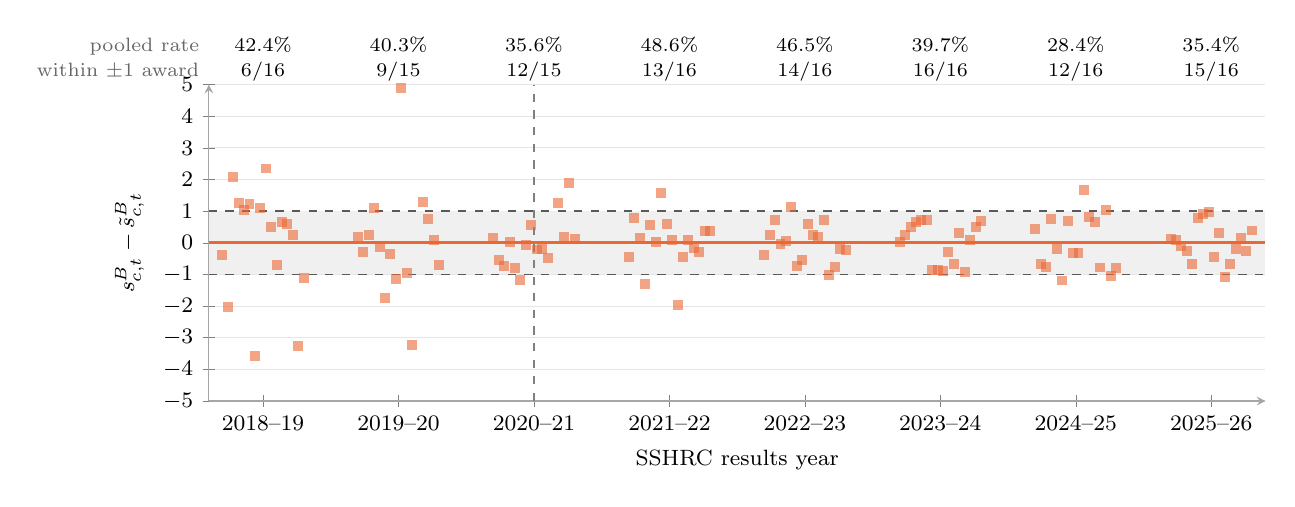
\begin{tikzpicture}
\begin{axis}[
  width=15cm, height=5.6cm,
  xmin=2017.6, xmax=2025.4, ymin=-5, ymax=5,
  xtick={2018,2019,2020,2021,2022,2023,2024,2025}, xticklabels={2018--19,2019--20,2020--21,2021--22,2022--23,2023--24,2024--25,2025--26},
  axis x line=bottom, axis y line=left, axis line style={gray!70},
  ymajorgrids, grid style={gray!20},
  tick label style={font=\footnotesize}, label style={font=\footnotesize},
  xlabel={SSHRC results year}, ylabel={$s^{B}_{c,t}-\tilde{s}^{B}_{c,t}$}, ylabel style={align=center},
  clip=false,
  ytick distance=1,
]
\fill[gray!12] (axis cs:2017.6,-1) rectangle (axis cs:2025.4,1);
\draw[gray, dashed, line width=0.7pt] (axis cs:2020,-5) -- (axis cs:2020,5);
\addplot[color=sshrcB, line width=1.2pt, forget plot, domain=2017.6:2025.4, samples=2] {0};
\addplot[gray!70!black, line width=0.7pt, dashed, forget plot, domain=2017.6:2025.4, samples=2] {-1};
\addplot[gray!70!black, line width=0.7pt, dashed, forget plot, domain=2017.6:2025.4, samples=2] {1};
\addplot[only marks, mark=square*, mark size=1.8pt, color=sshrcB,
  mark options={fill opacity=0.6, draw opacity=0}]
  coordinates {(2018.18,0.59) (2018.26,-3.26) (2018.06,0.50) (2018.10,-0.69) (2018.14,0.65) (2017.78,2.08) (2017.90,1.23) (2017.74,-2.02) (2018.30,-1.11) (2018.22,0.25) (2017.82,1.25) (2017.70,-0.39) (2018.02,2.35) (2017.94,-3.57) (2017.98,1.11) (2017.86,1.04) (2019.18,1.29) (2019.26,0.10) (2019.06,-0.96) (2019.10,-3.22) (2018.78,0.24) (2018.90,-1.74) (2018.74,-0.30) (2019.30,-0.71) (2019.22,0.74) (2018.82,1.11) (2018.70,0.18) (2019.02,4.89) (2018.94,-0.34) (2018.98,-1.14) (2018.86,-0.14) (2019.70,0.15) (2019.74,-0.54) (2019.78,-0.72) (2019.82,0.02) (2019.86,-0.79) (2019.90,-1.17) (2019.94,-0.08) (2019.98,0.56) (2020.02,-0.21) (2020.06,-0.20) (2020.10,-0.48) (2020.18,1.26) (2020.22,0.17) (2020.26,1.90) (2020.30,0.12) (2020.70,-0.46) (2020.74,0.77) (2020.78,0.14) (2020.82,-1.29) (2020.86,0.56) (2020.90,0.02) (2020.94,1.59) (2020.98,0.59) (2021.02,0.08) (2021.06,-1.95) (2021.10,-0.44) (2021.14,0.08) (2021.18,-0.15) (2021.22,-0.29) (2021.26,0.37) (2021.30,0.37) (2021.70,-0.39) (2021.74,0.24) (2021.78,0.73) (2021.82,-0.04) (2021.86,0.05) (2021.90,1.12) (2021.94,-0.74) (2021.98,-0.53) (2022.02,0.59) (2022.06,0.26) (2022.10,0.19) (2022.14,0.73) (2022.18,-1.02) (2022.22,-0.76) (2022.26,-0.20) (2022.30,-0.23) (2022.70,0.02) (2022.74,0.26) (2022.78,0.51) (2022.82,0.65) (2022.86,0.72) (2022.90,0.73) (2022.94,-0.85) (2022.98,-0.85) (2023.02,-0.89) (2023.06,-0.28) (2023.10,-0.68) (2023.14,0.32) (2023.18,-0.92) (2023.22,0.08) (2023.26,0.49) (2023.30,0.69) (2023.70,0.45) (2023.74,-0.68) (2023.78,-0.76) (2023.82,0.76) (2023.86,-0.20) (2023.90,-1.19) (2023.94,0.68) (2023.98,-0.31) (2024.02,-0.31) (2024.06,1.66) (2024.10,0.81) (2024.14,0.66) (2024.18,-0.78) (2024.22,1.05) (2024.26,-1.04) (2024.30,-0.80) (2024.70,0.11) (2024.74,0.10) (2024.78,-0.10) (2024.82,-0.25) (2024.86,-0.68) (2024.90,0.79) (2024.94,0.90) (2024.98,0.96) (2025.02,-0.46) (2025.06,0.32) (2025.10,-1.09) (2025.14,-0.68) (2025.18,-0.20) (2025.22,0.16) (2025.26,-0.26) (2025.30,0.39)};
\node[font=\scriptsize, anchor=base east, text=gray!80!black] at ([yshift=12pt]axis cs:2017.6,5) {pooled rate};
\node[font=\scriptsize, anchor=base] at ([yshift=12pt]axis cs:2018,5) {42.4\%};
\node[font=\scriptsize, anchor=base] at ([yshift=12pt]axis cs:2019,5) {40.3\%};
\node[font=\scriptsize, anchor=base] at ([yshift=12pt]axis cs:2020,5) {35.6\%};
\node[font=\scriptsize, anchor=base] at ([yshift=12pt]axis cs:2021,5) {48.6\%};
\node[font=\scriptsize, anchor=base] at ([yshift=12pt]axis cs:2022,5) {46.5\%};
\node[font=\scriptsize, anchor=base] at ([yshift=12pt]axis cs:2023,5) {39.7\%};
\node[font=\scriptsize, anchor=base] at ([yshift=12pt]axis cs:2024,5) {28.4\%};
\node[font=\scriptsize, anchor=base] at ([yshift=12pt]axis cs:2025,5) {35.4\%};
\node[font=\scriptsize, anchor=base east, text=gray!80!black] at ([yshift=3pt]axis cs:2017.6,5) {within $\pm1$ award};
\node[font=\scriptsize, anchor=base] at ([yshift=3pt]axis cs:2018,5) {6/16};
\node[font=\scriptsize, anchor=base] at ([yshift=3pt]axis cs:2019,5) {9/15};
\node[font=\scriptsize, anchor=base] at ([yshift=3pt]axis cs:2020,5) {12/15};
\node[font=\scriptsize, anchor=base] at ([yshift=3pt]axis cs:2021,5) {13/16};
\node[font=\scriptsize, anchor=base] at ([yshift=3pt]axis cs:2022,5) {14/16};
\node[font=\scriptsize, anchor=base] at ([yshift=3pt]axis cs:2023,5) {16/16};
\node[font=\scriptsize, anchor=base] at ([yshift=3pt]axis cs:2024,5) {12/16};
\node[font=\scriptsize, anchor=base] at ([yshift=3pt]axis cs:2025,5) {15/16};
\end{axis}
\end{tikzpicture}
